%\newpage
\section{Fermi smearing}
\mbox{}\vspace{-\baselineskip}

Let's now assume that for all events in the sample the reaction happens off a moving proton, as in the case when the proton is contained within a nucleus. Then the four-momentum of the target proton has the following components, 
\begin{equation}
\begin{aligned}
P_{p}^{\mu} = (\sqrt{m^{2}_{p}+p^{2}_{F}},~p_{F}^{x},~p_{F}^{y},~p_{F}^{z}),
\end{aligned}\label{eq:p_4mom}
\end{equation}
where $p_{F}^{j}$ ($j=x,~y,~z$) are the components of the proton three-momentum (or the Fermi-momentum) and $p_{F}$ is its magnitude. Note that the proton is assumed to be on mass-shell.

If for each event in the sample the components of the Fermi momentum are exactly known without any uncertainty, then $P_{p}^{\mu}$ given by Eq.~\eqref{eq:p_4mom} can be used to calculate the missing quantities $M_{X[0]}^{2}$ and $M_{X[\pi^{-}]}^{2}$. Such a calculation will then result in Eqs.~\eqref{eq:plain}, which correspond to the illustration in Fig.~\ref{fig:norad_nofsi}. 


However, for event samples collected experimentally, the information on the initial proton momentum is typically not accessible or incomplete, which leads to the inevitability to conduct the analysis under the target-at-rest assumption. This means that the following form of the initial proton four-momentum is used to calculate the missing quantities,
\begin{equation}
\begin{aligned}
\widetilde{P}_{p}^{\mu} = (m_{p},~0,~0,~0).
\end{aligned}\label{eq:p_4mom_rest}
\end{equation}

Now one can proceed to estimating the quantities $M_{X[0]}^{2}$ and $M_{X[\pi^{-}]}^{2}$ under the target-at-rest assumption. The former can be expressed by
\begin{equation}
\begin{aligned}
&M_{X[0]}^{2}&=&~\left [P_{X[0]}^{\mu} \right ]^{2}&=&~ \left (\widetilde{P}^{\mu}_{p} - P^{\mu}_{p} \right )^{2}=[\widetilde{P}^{\mu}_{p} ]^{2} + [P^{\mu}_{p}]^{2}-2 [\widetilde{P}_{p} ]_{\mu} P_{p}^{\mu}\\
&&&&=&~2m_{p}^{2}-2m_{p}\sqrt{m_{p}^{2}+p_{F}^{2}}=2m_{p}\left (m_{p} - \sqrt{m_{p}^{2}+p_{F}^{2}} \right ) < 0.
\end{aligned}\label{eq:mm0_fermi}
\end{equation}

The final expression in Eq.~\eqref{eq:mm0_fermi} depends on the Fermi momentum magnitude (but not on its direction) and is independent on the reaction kinematics. The $M_{X[0]}^{2}$ distribution thus acquires the left-sided smearing and kinematically stable shape.


%\begin{equation}
%\begin{aligned}
%2m_{p}^{2}-2m_{p}\sqrt{m_{p}^{2}+p_{F}^{2}}& ~~\wedge~~ 0&\\
%m_{p}^{2}& ~~\wedge~~ m_{p}\sqrt{m_{p}^{2}+p_{F}^{2}}&\\
%m_{p}^{4}& ~~\wedge~~ m_{p}^{2}(m_{p}^{2}+p_{F}^{2})&\\
%m_{p}^{4}& ~~\wedge~~ m_{p}^{4}+m_{p}^{2}p_{F}^{2}&\\
%0& ~~<~~ m_{p}^{2}p_{F}^{2}&
%\end{aligned}\label{eq:fermi_comp}
%\end{equation}

Meanwhile, the quantity $M_{X[\pi^{-}]}^{2}$ can be written in the following way,
\begin{equation}
\begin{aligned}
&M_{X[\pi^{-}]}^{2}&=&~\left [P_{X[\pi^{-}]}^{\mu} \right ]^{2}&=&~\left (P_{\pi^{-}}^{\mu}+ \widetilde{P}^{\mu}_{p} - P^{\mu}_{p} \right )^{2}\\
&&&& =&~\left [P^{\mu}_{\pi^{-}} \right ]^{2} + \left (  \widetilde{P}^{\mu}_{p} - P^{\mu}_{p} \right )^{2}+2[P_{\pi^{-}}]_{\mu} \left ( \widetilde{P}^{\mu}_{p}  -  P^{\mu}_{p}  \right )\\
&&&&=&~m_{\pi^{-}}^{2} + M_{X[0]}^{2} +2\left \{ E_{\pi^{-}}\left (m_{p}-\sqrt{m_{p}^{2}+p_{F}^{2}}\right ) + (\overrightarrow{p}_{\pi^{-}} \cdot \overrightarrow{p}_{F}) \right \}\\
&&&&=&~m_{\pi^{-}}^{2} + 2\left (m_{p}+E_{\pi^{-}}\right )\left (m_{p}-\sqrt{m_{p}^{2}+p_{F}^{2}}\right ) +2\left (\overrightarrow{p}_{\pi^{-}} \cdot \overrightarrow{p}_{F} \right ),\\
\end{aligned}\label{eq:mmpim_fermi}
\end{equation}
where for $M_{X[0]}^{2}$ the expression obtained in Eq.~\eqref{eq:mm0_fermi} was employed.

The final expression in Eq.~\eqref{eq:mmpim_fermi} depends on the magnitude and direction of the Fermi momentum as well as the reaction kinematics. It is also noteworthy that the second summand in this expression is always negative, while the third summand can have either sign. Thus, the value of $M_{X[\pi^{-}]}^{2}$ can be either greater or smaller than $m_{\pi^{-}}^{2}$, depending on the interplay between the two terms. All these lead to both-sided smearing of the $M_{X[\pi^{-}]}^{2}$ distribution and kinematic dependence of its shape.


\begin{figure}[htp]
\begin{center}
\framebox{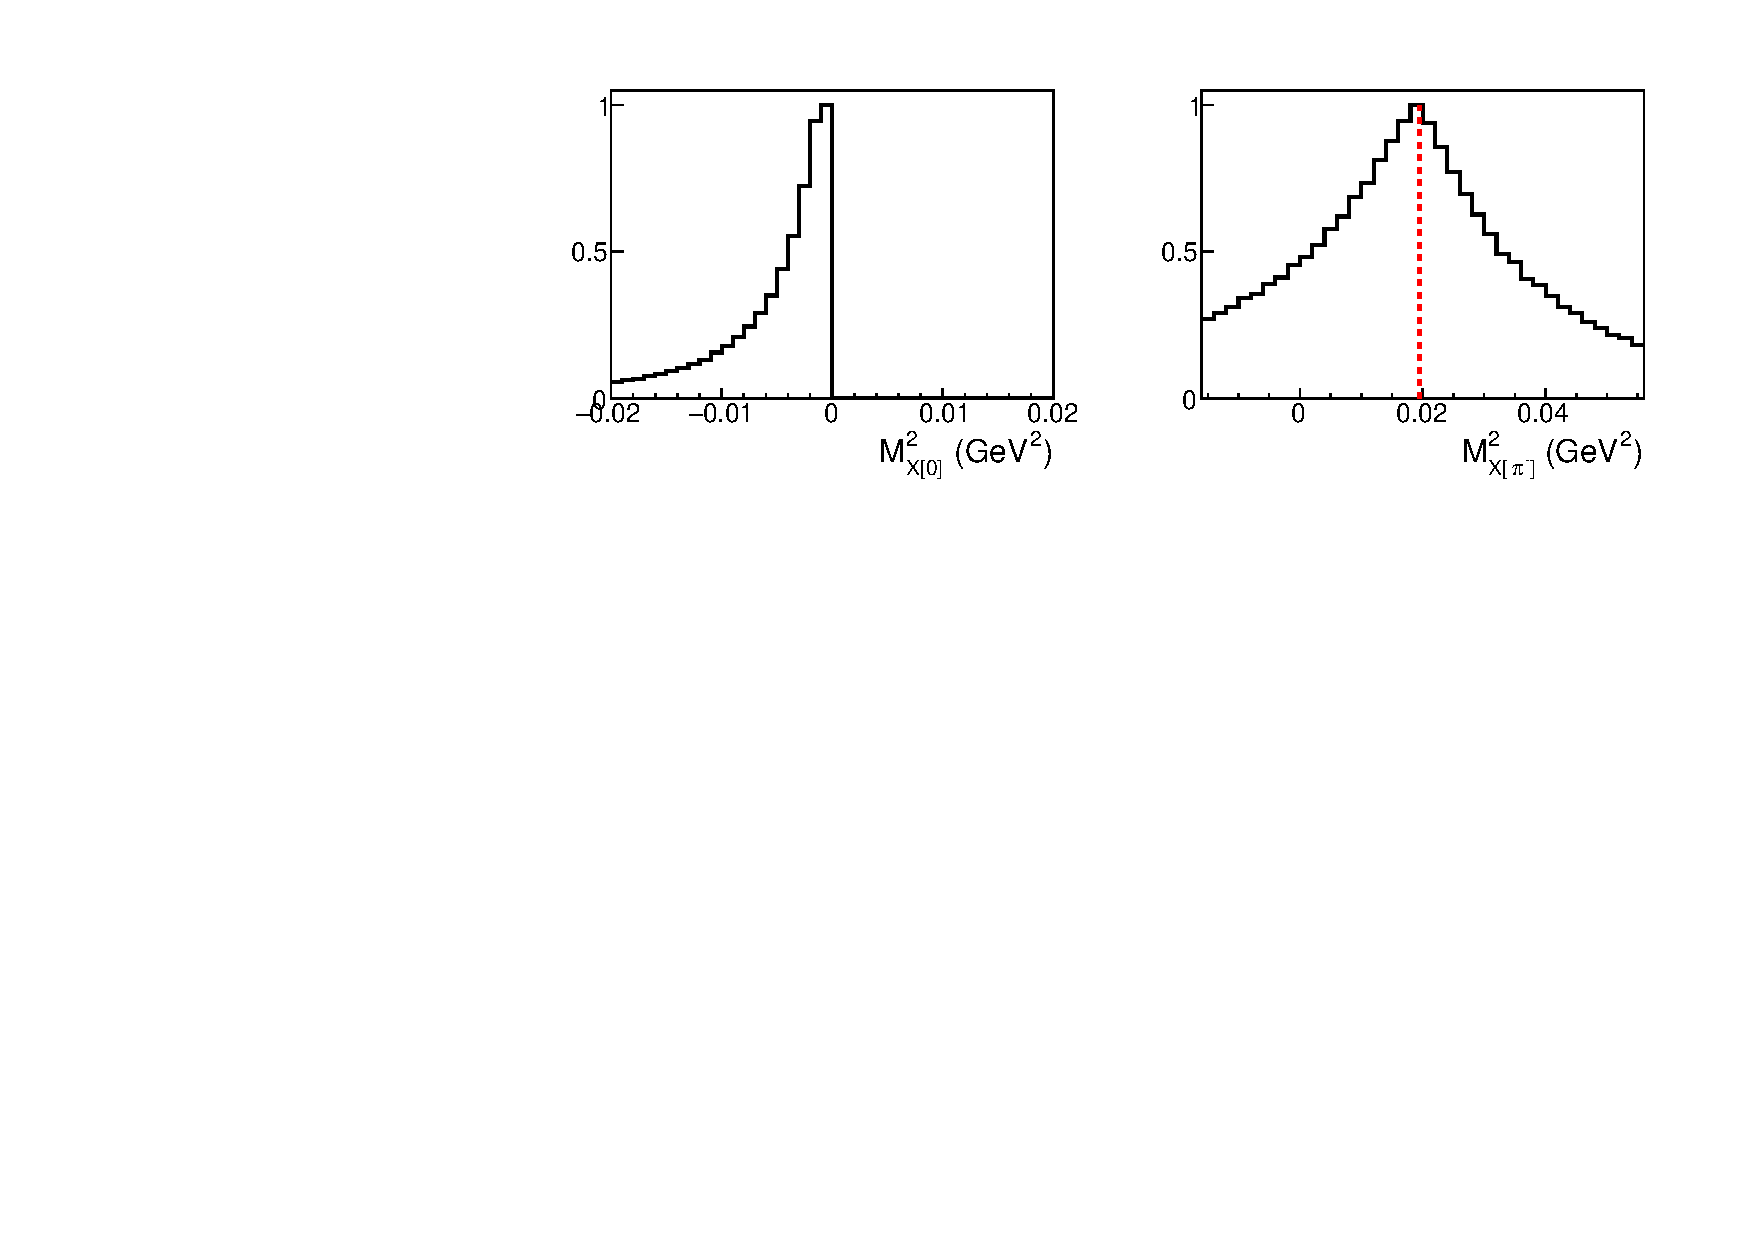
\includegraphics[width=\textwidth]{pictures/mm_fermi.pdf}}
\caption{\small Quantities $M_{X[0]}^{2}$ (left) and $M_{X[\pi^{-}]}^{2}$ (right) affected by the Fermi smearing. The distributions are plotted under the target-at-rest assumption for the reaction occurring off protons that move in deuterium nuclei. To produce the plots, the TWOPEG-D event generator~\cite{twopeg-d} was used, which assumes the reaction to happen in the quasi-free regime and the momentum of the initial proton to be distributed according to the Bonn potential~\cite{Machleidt:1987hj}. The red dashed line in the right plot marks the value of $m_{\pi^{-}}^{2}$.} \label{fig:mm_fermi}
\end{center}
\end{figure}

The foregoing calculations are illustrated in Fig.~\ref{fig:mm_fermi}, which shows the distributions of the missing quantities plotted under the target-at-rest assumption for the reaction occurring off protons that move in deuterium nuclei. These distributions are produced by the TWOPEG-D event generator~\cite{twopeg-d}, which assumes the reaction to happen in the quasi-free regime and the momentum of the initial proton to be distributed according to the Bonn potential~\cite{Machleidt:1987hj}. As seen in the plots, distributions of both missing quantities demonstrate a considerable Fermi smearing, which is left-sided for $M_{X[0]}^{2}$ and both-sided for $M_{X[\pi^{-}]}^{2}$. 

The kinematic dependence of the $M_{X[\pi^{-}]}^{2}$ distribution is worth special mentioning. For $W$ close to the threshold, its shape is strongly asymmetric with the event excess at the left. As $W$ grows, the asymmetry gradually vanishes, and at $W\sim $ 1.7-1.8~GeV the distribution becomes symmetric. In addition to that, the distribution smearing increases with growing~$W$. The plot in the right panel of Fig.~\ref{fig:mm_fermi} is produced for the $W$ range from 1.4~GeV to 1.8~GeV, and hence demonstrates the combined impact of these effects.


